% $Id: template.tex 11 2007-04-03 22:25:53Z jpeltier $
\documentclass{vgtc}                          % final (conference style)

\ifpdf%                                % if we use pdflatex
  \pdfoutput=1\relax                   % create PDFs from pdfLaTeX
  \pdfcompresslevel=9                  % PDF Compression
  \pdfoptionpdfminorversion=7          % create PDF 1.7
  \ExecuteOptions{pdftex}
  \usepackage{graphicx}                % allow us to embed graphics files
  \DeclareGraphicsExtensions{.pdf,.png,.jpg,.jpeg} % for pdflatex we expect .pdf, .png, or .jpg files
\else%                                 % else we use pure latex
  \ExecuteOptions{dvips}
  \usepackage{graphicx}                % allow us to embed graphics files
  \DeclareGraphicsExtensions{.eps}     % for pure latex we expect eps files
\fi%

%% it is recomended to use ``\autoref{sec:bla}'' instead of ``Fig.~\ref{sec:bla}''
\graphicspath{{figures/}{pictures/}{images/}{./}} % where to search for the images

\usepackage{microtype}                 % use micro-typography (slightly more compact, better to read)
\PassOptionsToPackage{warn}{textcomp}  % to address font issues with \textrightarrow
\usepackage{textcomp}                  % use better special symbols
\usepackage{mathptmx}                  % use matching math font
\usepackage{times}                     % we use Times as the main font
\renewcommand*\ttdefault{txtt}         % a nicer typewriter font
\usepackage{tabu}                      % only used for the table example
\usepackage{booktabs}                  % only used for the table 
\usepackage{url}
\usepackage{tabularray}
\usepackage[backend=biber]{biblatex}
\addbibresource{template.bib}

\onlineid{0}
\vgtccategory{Research}

\title{The state-of-art
platforms and tools which can be used to develop immersive analytical
applications}

\author{Walid Chtioui\thanks{e-mail: walid.chtioui@ensi-uma.tn}\\ %
        \scriptsize University of Passau %
\and Achraf Hebheb\thanks{e-mail: habhabachref@gmail.com}\\ %
     \scriptsize University of Passau}

%% A teaser figure can be included as follows, but is not recommended since
%% the space is now taken up by a full width abstract.
%\teaser{
%  \includegraphics[width=1.5in]{sample.eps}
%  \caption{Lookit! Lookit!}
%}

\abstract{This paper presents an overview of the latest state-of-the-art
platforms and tools which can be used to develop immersive analytics
(hereafter IA) applications. The term platform refers to programs that provide
a high-level application programming interface (API) along side a set
of extensive XR features which allow developers to create complex XR
experiences. Initially, an overview of what we believe are the major extended
reality (hereafter XR) development platforms is provided after which a table
of, what we think are, important-to-have features and by which platforms they
are supported is presented.
} % end of abstract

\CCScatlist{ 
    {HEY}{HEY}
}

%%%%%%%%%%%%%%%%%%%%%%%%%%%%%%%%%%%%%%%%%%%%%%%%%%%%%%%%%%%%%%%%
%%%%%%%%%%%%%%%%%%%%%% START OF THE PAPER %%%%%%%%%%%%%%%%%%%%%%
%%%%%%%%%%%%%%%%%%%%%%%%%%%%%%%%%%%%%%%%%%%%%%%%%%%%%%%%%%%%%%%%%

\begin{document}
\firstsection{Introduction}
\maketitle
This template is for papers of VGTC-sponsored conferences which are
\emph{\textbf{not}} published in a special issue of TVCG.

\section{Platforms}
\subsection{Unity}
Unity has a wide adoption in the world of XR thanks to its unified workflow
and support for various XR platforms - build once, run
everywhere -. Unity supports an extensive set of XR vendor-specific software
development kits (hereafter SDK) including: Apple's ARKit, Google's ARCore,
Microsoft's HoloLens and OpenXR. Following the announcement of Apple's
mixed reality (MR) headset Vision Pro in Apple's Worldwide Developers
Conference (WWDC) 2023, Unity was announced to provide native support for
Vision's Pro operating system VisionOS \cite{web:vision_pro_unity}.
Unity also provides a set of XR packages that are built on top of these vendor
plugins to add application-level development tools \cite{unity:xr_packages}.
For instance, AR Foundation is an industry-standard framework that provides
support for various AR features such as: object tracking and plane detection.
\subsection{Unreal Engine}
\subsection{Comparison}
Figure \ref{table:1} provides a comparison between the previously discussed
platforms in terms of support for vendor-specific SDKs and a set of features.

\begin{table}[h!]
	\centering

	\begin{tabular}{l c c}
		\toprule
		                     & \multicolumn{2}{c}{\textbf{Platform}}                     \\
		\cmidrule(l){2-3}
		\textbf{SDKs}        & Unity 2022 LTS                        & Unreal Engine 5.3 \\
		\midrule
		ARCore               & X                                     & X                 \\
		ARKit                & X                                     & X                 \\
		Magic Leap           & X                                     & X                 \\
		Microsof HoloLens    & X                                     & X                 \\
		OpenXR               & X                                     & X                 \\
		Oculus               & X                                     & X                 \\
		WebXR                & X                                     &                   \\
		VisionOS             & X                                     &                   \\
		\midrule
		\textbf{AR Features} &                                       &                   \\
		\midrule
		Plane Detection      & X                                     & X                 \\
		Object Occlusion     & X                                     & X                 \\
		Environment Probes   & X                                     & X                 \\
		Face Tracking        & X                                     & *(ARKit only)     \\
		Object Tracking      & X                                     & X                 \\
		Body Tracking        & X                                     & ? (not mentioned) \\
		Camera Intrinsics    & X                                     & X                 \\
		Meshing              & X                                     & ? (not mentioned) \\
		\midrule
		Vuforia Support      & X                                     &                   \\
		\bottomrule
	\end{tabular}


	\medskip

	\caption{Per-platform supported SDKs, AR features and 3rd party tools.}
	\label{table:1}
\end{table}

\section{Toolkits and Frameworks}

TODO: add what do we mean by 'toolkit' + what will be discussed here

\subsection{DXR Toolkit}

Sicat et al. proposed DXR \cite{dxr_toolkit}; an IA toolkit built on top of the Unity game engine
that allows fast prototyping and iteration for non-experienced users; i.e.
users with no or little programming knowledge in XR and Unity.
Alongside the data input, DXR takes a specification file written in JavaScript
Object Notation (hereafter JSON) from which visualisations are created.
The specification file is described in Vega-Lite declarative grammar \cite{vega_lite}
(only what should be achieved has to be provided, not how) making it suitable
for users with no programming experience to rapidly realise immersive
visualisations. This file can be edited in a separate text editor or through
the use of a GUI with pre-configured set of parameters. DXR also provides
built-in specification templates for common visualisations such as: Scatter
plots and bar charts. This extends the scope of users even more to include
those without any technical experience. Although the authors claim that DXR
provides suitable flexibility, the scope of that flexibility seems to be
limited, among other things, to providing custom graphical markers, custom
encoding channels - a visualization channel is a visualisation parameter affected by some
data dimension(s), such as object color affected by temperature data dimension in some dataset -
and other visualisation-type specific properties. That limits users to a
templated and common set of visualisations such as scatter plots, bar charts
and radial bars. There is also no mention of real-time data support thus
limiting the use case of DXR to offline data only.

\smallskip

\noindent As the authors have explicitly mentioned, DXR is meant for
prototyping and exploring designs, it is not designed to handle visualisations
of large datasets. On HoloLens, for datasets with more than approximately
a thousand item, suboptimal - less that 60 frames per second (hereafter FPS) -
performance has been observed. Nonetheless, the authors argue that DXR can still
be useful for quickly and cheaply prototyping large dataset designs before
moving to specialized, optimized and detailed implementations.

\subsection{IATK Toolkit}
Maxime et al. introduced IATK \cite{iatk_toolkit}; an open-source software
package for Unity that provides both a high-level Unity-editor-integrated GUI
for simple authoring and a low-level C-sharp and JavaScript API for
fine-grained authoring and extending the visualizations.

To some degree of similarity to DXR, IATK relies on a high-level declarative
grammar of graphics by providing a composable grammar of visualization
primitives alongside a high-level interface for rapid prototyping and
iterations. What sets IATK apart, is that it was designed with scalability in
mind, a focus on large and complex datasets and a focus on user interactions.
The toolkit's authors claim that it can render millions of items thanks to its
use of efficient GPU shader code. Also, contrary to DXR, IATK does not support
declarative configurations it instead relies on a Unity editor GUI or C-sharp
API code that make use of a composable grammar to author visualizations.

\begin{figure}[tb]
	\centering
	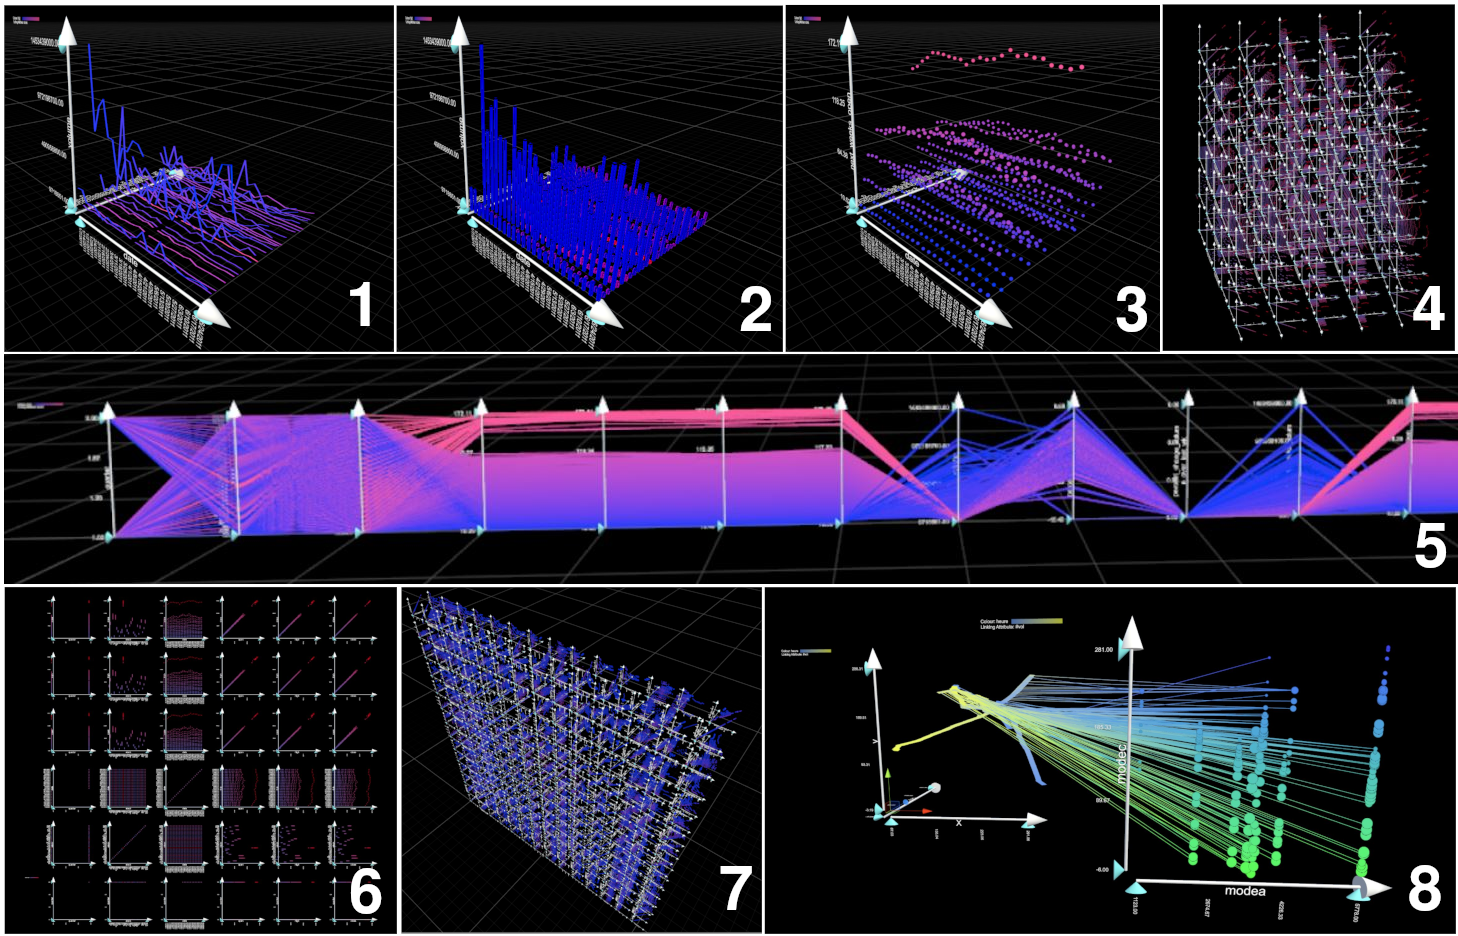
\includegraphics[width=\columnwidth]{iatk}
	\caption{IATK visualizations. (1) 3D scatter plot with sphere datapoint
		geometry. The images are from is in the public domain.}
	\label{fig:sample}
\end{figure}

Unlike DXR and other toolkits built on top of Unity, IATK doesn't render
the datapoints (here we don't mean point as in a geometrical point) as Unity
game objects and use expensive-to-update-at-large-scale object attributes as
visualization channels. Instead, all the datapoints are visualized within one
game object where each data point is encoded into a unique vertex by mapping
data attributes, such as position, color and size, into vertex components such
as vertex UV coordinates which is a two dimensional vector, vertex normal vector
and vertex color. This way, actual datapoint geometries are created on the GPU
resulting in a what is claimed to be more efficient rendering process. This
however greatly limits the customizability of datapoint marks and the choice
of visualization channels.

According to the authors' performance statistics, on VR less than 90 FPS is
observed at two million datapoints and on AR less than 60 FPS is observed at
just a thousand datapoints. However, one can subjectively claim that the performance on AR
HoloLens headset remains acceptable up-to ten thousand datapoints at which 41
FPS is achieved. Although the authors provided FPS statistics for Oculus CV1,
Meta2 and HoloLens devices, no performance statistics were provided for the
alternative game-object-based datapoint approach to provide a performance
reference point.

IATK integrates an interactive visualization model within its visualization
components that allows a set of interactions including filtering, brushing and
linking, details on demand, animated transitions and attribute-based animations.
These interactions are implemented in the vertex shader part of the rendering
pipeline which leverages the high parallelism nature of the GPU(s) making them
particularly responsive and efficient at handling large datasets.

IATK's high-level GUI provides just three built-in visualization types:
either a scatterplot, a parallel coordinates or a scatterplot matrix. It also
only provides a small set of datapoint geometries. To extend these, one has to
use the provided low-level API which might limit expressiveness for
non-experienced users.

The authors didn't mention any support for neither real-time data
visualization nor local or remote collaboration. It is also worth mentioning
that for VR only scatterplot visualization type is supported. This greatly
limits the expressiveness for VR users.

\subsection{VRIA Toolkit}
Peter et al. introduce VRIA \cite{vria_framework}; a free and open-source
framework for building IA experiences in VR. Unlike the aforementioned
toolkits, VRIA isn't built as an add-on on top of a game engine. Instead, it is
built upon open-standard Web-based frameworks such as WebVR, A-Frame, React and
D3.js, all of which are mature, open-source and widely used Web-based
frameworks and libraries. This allows VRIA applications to be accessible by a
plethora of VR and non-VR devices.

\smallskip

\noindent The toolkit is designed to be accessible to novices and experts
alike. Similar to DXR, VRIA makes use of a declarative grammar based on
Vega-Lite to allow users to create custom visualizations based on configuration
files. However, this visualization configuration file is only required for
basic functionalities. For extra custom functionalities such as a custom set of
visualization channels, interactions, graphical marks or visualization types,
more experienced users can create these by using the provided low-level API.
VRIA provides The VRIA Builder; a Web application intended for beginners that
integrates a GUI and a 3D scene view to rapidly prototype visualization designs
with instant feedback without having to leave the browser. It is worth
mentioning that, unlike DXR, this customization GUI isn't part of the VR scene
and cannot be viewed withing the VR headset and only the scene view can be
experienced immersively. However, the authors mentioned their willingness to
add \textit{in-situ} GUI so that users can build and prototype visualizations
iteratively without having to remove the headset.

\smallskip

\noindent Thanks to its composable structure, the toolkit can be integrated into
other existing 2D or immersive visualization applications. For instance,
VRIA's visualizations can be overlaid on top of another A-Frame scene.
VRIA has support for collaborative immersive analytics through either the
high-level networking abstraction layer provided by the open-source Networked
A-Frame component or by using the provided API with lower-level networking
libraries.
In term of data input, the toolkit only supports tabular data in the form of
JSON or CSV thus real-time data visualization isn't supported. The authors
expressed their willingness to add support for other forms of data such as
geospatial GeoJSON, network and relational data models.

\smallskip

\noindent The authors stated that VRIA offers the option to integrate D3.js
visualization within its IA experiences. D3.js is web-base JavaScript
visualization library that provides a low-level approach to author graphics and
powerful mechanisms to transform and manipulate data. Since D3.js is widely
adopted, integrating it within VRIA allows for easier usability and quicker
authoring of 2D visualizations. However, there wasn't a detailed description of
which D3.js functionalities and visualizations are integrable nor any guidance
on how to integrate it within VRIA framework.

\smallskip

\noindent More experienced users seeking for a more custom experience are
forced to deal with two separate tools to author custom visualizations;
the visualization configuration file specified in a declarative language and
the API specified in JavaScript. We believe that it would be easier for the end users if VRIA
provided more customizability through the vis config file instead of just
providing very basic functionalities. We also question the necessity of adding
the extra A-Frame layer, albeit thin, on top of Three.js. A-Frames'
functionalities could be directly implemented in Three.js thus reducing and
simplifying the VRIA stack. But we do understand that A-Frame simplifies the
process of creating VR experiences on the web relative to the lower level
Three.js library. The authors stated their intention to work at the Three.js
level directly without any further abstraction libraries.

\smallskip

\noindent Whenever 3D graphics are mentioned in the context of web browsers,
performance implementations are one of the most worrying aspects. This is
especially true for Web-based VR applications where two images have to be
rendered each frame preferably at 90 FPS to avoid motionsickness. VRIA's
authors provided visualization benchmarks on a desktop monitor, a desktop
Oculus Rift CV1 and a smartphone. A scatter-plot visualization type was used
with sphere graphical marks. The exact set of visualization channels used
wasn't mentioned neither were attributes of the input data. On the desktop
monitor and Oculus Lift HMD, performance drops significantly after one
thousand data points. On smartphone performance starts dropping at one hundred
data points. This proves that VRIA is not suitable for large dataset
visualizations. The authors claim that the performance observed for the HMD
is similar to that of IATK for the HoloLens device. But the HoloLens uses
its own, much less powerful, hardware while VRIA performance benchmark used
the Oculus Lift CV1 VR HMD which relies on a separate desktop for expensive
rendering operations. We therefore question such comparisons of performance
benchmarks. This is later Web-based XR solutions do not compete,
in terms of performance, with game-engine based solutions.

\smallskip

\noindent VRIA only support Cartesian plots but the authors expressed their
willingness to add support for other coordinate systems including geographical
and spherical coordinates.
Moreover, although the authors showcased the ease of integrating VRIA with
AR.js to target AR experiences, the absence of an out-of-box support for VRIA
still limits AR accessiblity only to experienced users.

\subsection{Comparison}

\section{Prototypes}
\subsection{Uplift}
Barrett et al. proposed Uplift \cite{uplift_prototype}; an in-place
collaborative visual analytics prototype targeting users with diverse
expertise in the domain of microgrids. Uplift is designed for casual visual
analysis use-cases; i.e. to be used to easily identify, in a relatively short
time, key patterns in complex visualized data. The requirements for the
prototype were initially provided and subsequently modified, through multiple
feedback sessions, by a wide range of stakeholders including microgrid project
and energy systems experts.

\smallskip

\noindent Uplift relies more than just AR headsets to bring casual collaborative visual
analytics to a multitude of microgrid stakeholders. A tabletop display showing
a geographical map of the campus grid is used as a central platform where users
are supposed to gather around and interact with widgets placed on top of it.
Uplift also makes use of tangible
widgets which are physical and interactive elements that control visualization
parameters (for instance by affecting sliders). The prototype also relies on
scaled-down physical models of buildings that are translucent which allows
the color of the surface on which they are placed to be used as an appealing
visualization channel. AR is used to display multiple 3D data types on top of
the tabletop and 2D graphs alongside legends around it. On top of these, Uplift
uses a large display to either replicate the content of the tabletop or show
additional visualizations.

\smallskip

\noindent Through the feedback of 16 participants who tried the prototype, Uplift was
proven to be potentially useful for microgrid-related data analytics.

\smallskip

\noindent Although Uplift was designed for microgrid-related systems,
the authors claim that its applicability domain can be extended to include
other domains that rely on analysis of complex spatial data such as
the construction industry. However, the use of a wide range of technologies
and gadgets makes Uplift a specialized solution that we believe isn't yet
ready for wide deployment. For instance, on top of using Vuforia for tabletop
tracking, Uplift uses an extra proprietary tracking software with four cameras
to track the tangible widgets. Such tracking could have instead been done in
Vuforia therefore removing the need to add cameras to the scene and making the
solution much more self-contained. This is especially true since Vuforia provides
an official plugin for Unity development \cite{unity:vuforia_plugin}.
Moreover, although the topic of real-time monitoring of the microgrid was seen
as beneficial for operators by expert stakeholders, Uplift didn't provide any
solutions to tackle such use case.

\section{Collaboration Tools and Techniques}
\section{Interaction Tools and Techniques}
\section{Navigation Tools and Techniques}

\section{Conclusion}
TO BE WRITTEN AT THE VERY END

\acknowledgments{TO BE WRITTEN AT THE VERY END}
\printbibliography
\end{document}
